\documentclass[10pt]{article}
\usepackage[polish]{babel}
\usepackage[utf8]{inputenc}
\usepackage[T1]{fontenc}
\usepackage{amsmath}
\usepackage{amsfonts}
\usepackage{amssymb}
\usepackage[version=4]{mhchem}
\usepackage{stmaryrd}
\usepackage{graphicx}
\usepackage[export]{adjustbox}
\graphicspath{ {./images/} }

\title{Zadania - etap III (szkoła podstawowa) }

\author{}
\date{}


\begin{document}
\maketitle
Zadanie 1. Ile stopni ma kąt \(C A D\) w figurze na poniższym rysunku?\\
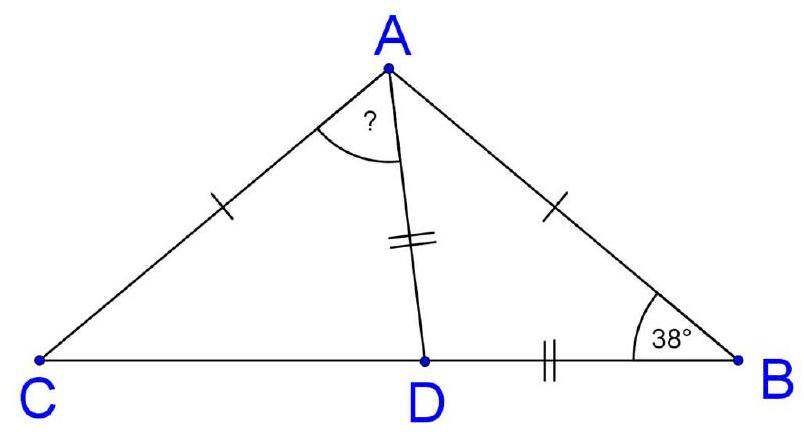
\includegraphics[max width=\textwidth, center]{2024_11_21_4c6a68efbf7bb0941ed2g-1(1)}

Zadanie 2. Oblicz wartość wyrażenia: \(\frac{3^{4}-9^{2}+10^{0}}{0,(6) \cdot 0,(2)}\).

Zadanie 3. W narożnikach trójkąta równobocznego o boku długości 8 cm odcięto trzy małe trójkąty równoboczne o tych samych długościach boków. Okazało się, że suma obwodów tych trzech małych trójkątów jest równa obwodowi pozostałego, zakreskowanego sześciokąta . Ile wynosi długość boku w małych trójkątach?\\
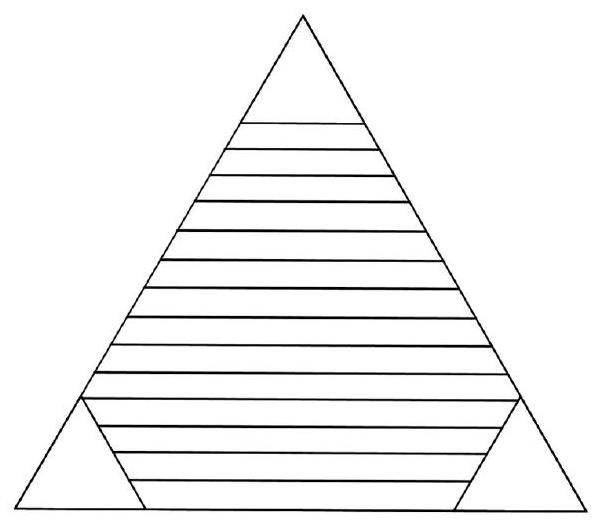
\includegraphics[max width=\textwidth, center]{2024_11_21_4c6a68efbf7bb0941ed2g-1}

Zadanie 4. Marysia wybrała sobie pewną liczbę. Dodała do niej \(3 \cdot 10^{2}\), a następnie wynik pomnożyła przez \(\left(2^{3}-5\right)\), a potem odjęła \(5^{2}\). Rezultat zmniejszyła \(2^{3}\) razy i otrzymała liczbę \(10^{2}\). Jaką liczbę wybrała Marysia na początku?

Zadanie 5. W pensjonacie nadmorskim „Pod różą" jest łącznie 70 miejsc noclegowych w pokojach dwuosobowych i trzyosobowych. Wszystkich pokoi jest 29. Ile jest pokoi dwuosobowych, a ile trzyosobowych w tym pensjonacie?


\end{document}